\documentclass[]{article}
\usepackage[utf8]{inputenc}
\usepackage[spanish]{babel}
\usepackage{graphicx}
\usepackage{color}
\usepackage[usenames,dvipsnames,svgnames,table]{xcolor}
\usepackage{hyperref}
\usepackage{url}
\usepackage{listings}
\hypersetup{
	colorlinks   = true,
	citecolor    = gray,
	urlcolor     = darkgray,
	linkcolor	 = darkgray
}

%opening
\title{Sistemas Inteligentes para la Gestión en la Empresa\\-\\Práctica 2: Deep Learning para multi-clasificación}
\author{Carlos Cobos Suárez\\Adrián Morente Gabaldón}

\begin{document}

\maketitle
\newpage
\tableofcontents
\newpage

\section{Introducción}

En este proyecto vamos a realizar diversas aproximaciones al tratamiento de técnicas de \textbf{aprendizaje profundo} con el lenguaje \textbf{\textit{R}}. Tras ponernos en situación con los fundamentos teóricos necesarios para entender el desarrollo realizado, comentaremos las soluciones pensadas y las que finalmente se hayan implementado; realizando después una discusión de los resultados obtenidos.\\

El conjunto de datos (o \textit{dataset}) que utilizaremos se corresponde con el de \textbf{\textit{PetFinder.my Adoption Prediction}}, y podemos encontrarlo en la plataforma \href{https://kaggle.com}{Kaggle} \cite{petfinder-dataset}. Los datos contenidos clasifican un histórico de perros y gatos alojados en centros de adopción de animales, con diversas características y almacenando el \textbf{tiempo de adopción} de cada una de estas mascotas.\\

El trabajo a desarrollar en este proyecto versa sobre el \textbf{entrenamiento de modelos de predicción} que, a partir de imágenes o de un conjunto de características de animales, clasifiquen éstos por tiempo de adopción. Para dicha clasificación, utilizaremos \textbf{cinco categorías} (las cuales se ordenan según el tiempo de adopción en orden ascendente). Lógicamente, la finalidad del trabajo será la de obtener la mejor precisión general posible, para lo que utilizaremos distintos modelos basados en \textbf{aprendizaje profundo}.\\

Dado que para el entrenamiento se dispone de un gran conjunto de datos ya clasificado, realizaremos algún \textbf{histograma}, lo que trata de un gráfico de barras que muestra el cardinal del conjunto de datos de cada una de las distintas categorías mencionadas.\\

Por otro lado, realizaremos también un \textbf{trabajo de investigación} relacionado con la aplicación de \textbf{técnicas de binarización}, planteando un marco teórico y comentando las distintas posibilidades que ofrecen.

\section{Fundamentos teóricos}

	Para entender tanto la finalidad del proyecto como los pasos realizados para su compleción, debemos ubicarnos en un marco teórico apropiado. Para empezar, antes de abordar la temática relacionada con el \textbf{aprendizaje profundo}, debemos hablar del \textbf{aprendizaje automático} y las técnicas más destacadas para su puesta en uso, como pueden ser las \textbf{redes neuronales} de diversos tipos.
	
	\subsection{Redes neuronales}
	
		Sabemos que la unidad básica de una red neuronal es, lógicamente, la \textbf{neurona}; cuya función es recibir unos datos de entrada, procesarlos mediante algunas operaciones matemáticas, y producir una salida.\\
		
		Estas entradas pueden provenir de la entrada al sistema o de la salida por parte de otras neuronas. Además, el número de éstas es variable, como podemos ver en la figura \ref{neuron}, donde se visualiza un ejemplo de neurona con dos entradas y una salida \cite{introduction-neural-networks}.\\
	
		\begin{figure}[h]
			\centering
			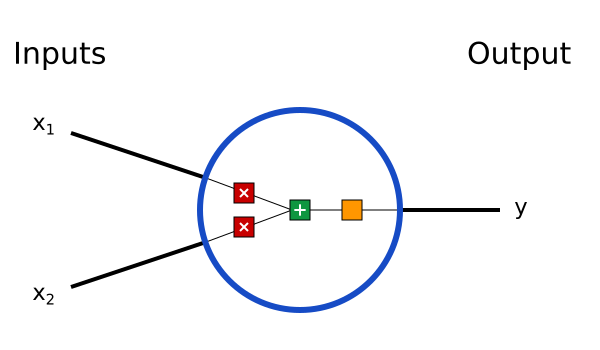
\includegraphics[width=0.5\textwidth]{./img/neuron}
			\caption{Neurona simple con dos entradas y una salida.}
			\label{neuron}
		\end{figure}
	
		Como se podría esperar a raíz de su nombre, sabiendo lo que es una neurona, podemos esperar que una \textbf{red neuronal} sea un conjunto conectado de varias neuronas. Podemos ver un ejemplo en la figura \ref{neural-network}.\\
		
		\begin{figure}[h]
			\centering
			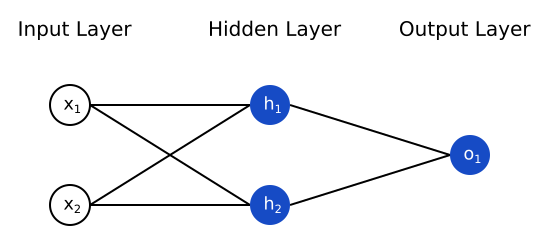
\includegraphics[width=0.5\textwidth]{./img/neural-network}
			\caption{Red neuronal simple con dos entradas y una salida.}
			\label{neural-network}
		\end{figure}
	
		Como podemos observar en dicha figura \ref{neural-network}, la red consta de una capa de entrada con dos neuronas, una red intermedia con otras dos, y finalmente de la capa de salida. Debemos saber que en dicha capa intermedia es donde se realizan sobre los datos de entrada todas las operaciones matemáticas que comentábamos anteriormente.\\
		
		Además, ha de destacarse que la conexión entre las neuronas de la red viene determinada por unos \textbf{pesos numéricos característicos}. Estos pesos son los que se utilizan a la hora de hacer el cálculo de salida final, dando una mayor importancia a ciertas neuronas con respecto a otras.\\
		
		Finalmente, en la capa de salida se combinan como entradas las salidas de la capa intermedia para, mediante una \textbf{función de activación}, producir una determinada salida.
		
	\subsection{Redes neuronales para tratamiento de imágenes}
	
		Conociendo las redes neuronales simples, debemos saber que \textbf{no son apropiadas para su uso con imágenes} debido a lo siguiente \cite{intro-convolutional-nn}:
		
		\subsubsection*{Tamaño de las imágenes}
		
			Los píxeles de una imagen son los que han de introducirse como entradas a la primera capa de una red neuronal. Si una imagen consta de 150 píxeles en blanco y negro, existirán 150 entradas. Si la imagen es a color (en modo \textit{RGB}), el número de entradas se multiplican por los tres canales de dicho formato.\\
			 
			Esto quiere decir que si una imagen consta de millones de píxeles, como encontramos actualmente en las tomadas por un teléfono móvil cualquiera, tendríamos que entrenar \textbf{millones de pesos} en la primera capa, lo que es prácticamente imposible en cualquier ordenador del que dispongamos.
			 
		\subsubsection*{Posición de las imágenes}
		
			Aunque en dos imágenes se muestre el mismo objeto para cuya detección ha sido entrenada la red neuronal simple, con una de este tipo no se es capaz de detectar que dicho objeto pueda cambiar en el espacio mostrado por la imagen. Es decir, aunque aparezca la misma cara humana que en otra imagen antes estudiada, que este elemento cambie de posición en la imagen implica que no sean las mismas neuronas las que se activen, por lo que el resultado de salida puede (y con mucha probabilidad) no ser el esperado.
			
		\subsubsection*{Solución}
		
			La solución para estos problemas la encontramos en las \textbf{redes neuronales de tipo convolucional}, que no son más que redes simples como las ya estudiadas pero que utilizan unas capas especiales, llamadas \textit{convolucionales}.\\
			
			Una \textbf{convolución} no es más que un filtro aplicado de forma iterativa a la imagen en forma de pequeña matriz de dos dimensiones. Un ejemplo práctico lo podemos ver en la referencia \cite{intro-convolutional-nn}, que aplica un \textbf{filtro horizontal de \textit{Sobel}} para mostrar la detección de límites en una imagen.\\
			
			En este caso el filtro usado (o \textit{kernel}) se muestra en la figura \ref{conv-filter}. Adicionalmente, en la figura \ref{conv-filter-result} se visualizan a la izquierda la imagen original sobre la que se aplica el filtro, y a su derecha la imagen resultante. Como podemos ver, el resultado es una nueva fotografía en blanco y negro donde se manifiestan los límites más relevantes de dicha foto.\\
			
			\begin{figure}[h]
				\centering
				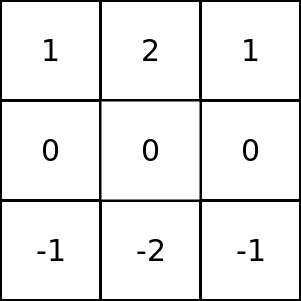
\includegraphics[width=0.2\textwidth]{./img/horizontal-sobel}
				\caption{Ejemplo de matriz de convolución - Filtro horizontal de \textit{Sobel}.}
				\label{conv-filter}
			\end{figure}
		
			\begin{figure}[h]
				\centering
				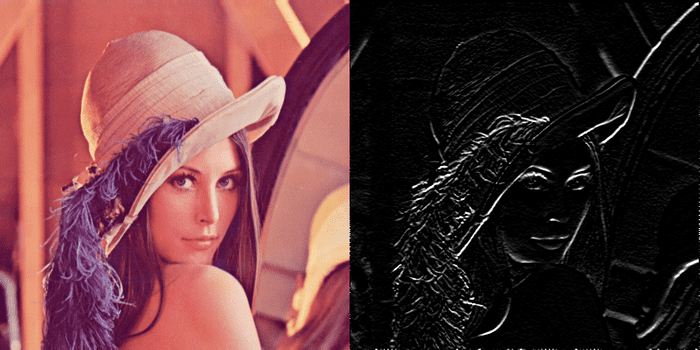
\includegraphics[width=0.6\textwidth]{./img/lenna+horizontal}
				\caption{Imagen original y su resultante tras aplicar el filtro convolucional de \textit{Sobel}.}
				\label{conv-filter-result}
			\end{figure}
		
			Utilizando la detección de límites de forma previa al entrenamiento de la red, se delimitan mucho mejor los elementos contenidos en la imagen, por lo que se favorece mucho dicha fase de aprendizaje.
	
	\subsection{\textit{Deep Learning}}
	
		Se conoce como \textbf{aprendizaje profundo} al campo de aplicación del \textbf{aprendizaje automático} donde se hace un uso más extenso de técnicas basadas en \textbf{redes neuronales artificiales}. Estas redes utilizadas son capaces de aprender \textit{profundamente} para trabajar con problemas como reconocimiento de imágenes, de texto o de voz; además de otras aplicaciones como filtrado colaborativo en redes sociales y visión por computador.\\
		
		La diferencia principal entre una red neuronal simple y las redes de \textit{aprendizaje profundo} reside en que las primeras, como ya hemos visto anteriormente, contienen una suma de tres capas: la de \textbf{entrada}, la \textbf{intermedia} (donde se aplican las operaciones) y la de \textbf{salida}.\\
		
		Por otro lado, en las redes neuronales de \textit{deep learning} el número de capas intermedias es mayor, con lo que se consigue un mejor aprendizaje. Esto se debe a que el número de neuronas (y por tanto de pesos en el modelo final) es mayor; y cuanto más alto sea el número de hiperparámetros presentes en un algoritmo, mayor es la capacidad de entrenamiento que tendrá dicho modelo final.\\
		
		\begin{figure}[h]
			\centering
			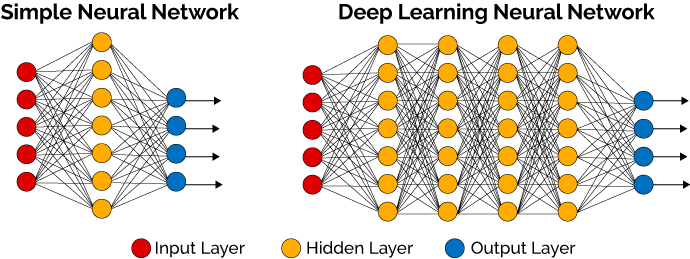
\includegraphics[width=0.8\textwidth]{./img/neural-network-differences}
			\caption{Diferencia entre red neuronal simple y red de aprendizaje profundo.}
			\label{nn-differences}
		\end{figure}
	
		\subsubsection*{Clasificación categórica}
		
			La finalidad de cualquier técnica de clasificación (o \textit{clustering}) es lógicamente asignar una clase concreta a cada una de las entradas. Esta clasificación podría ser \textbf{binaria} (si existen tan solo dos clases) o \textbf{multicategórica} (si existen más de dos).\\
			
			El problema de las clasificaciones multicategóricas es que pueden no detectar demasiado bien las características de cada clase y el modelo resultante puede errar con alta frecuencia en sus predicciones. Este problema también se evidencia con la existencia de un desequilibrio en el número de datos de cada clase encontrados en la fase de entrenamiento.\\
			
			Una forma de intentar poner solución a este problema es el uso de \textit{técnicas de binarización}, las cuales comentaremos en el apartado siguiente.
	
		\subsubsection{Técnicas de binarización}
		
			Al igual que en los métodos del tipo \verb|"divide y vencerás"|, surgen como técnica basada en la descomposición de un problema en otros de menor dimensión, de forma que en un problema de \textit{clustering}, no encontramos más de dos clases a la vez (clasificación binaria). Como podría esperarse, surge la necesidad de combinar las distintas salidas de cada uno de los nuevos clasificadores para así realizar la predicción final de clase (lo que se conoce como \textbf{agregación}). Veremos las técnicas de agregación más adelante.\\
			
			Según podemos ver en la referencia \cite{binary-classifiers}, artículo escrito por un grupo de investigación de profesores de nuestra propia facultad, existen dos técnicas de binarización principales: \textit{\textbf{One-vs-One}} y \textit{\textbf{One-vs-All}}, que describimos a continuación:\\
			
			{\large \textbf{\textit{One-vs-One}}}: Se basa en el uso de un clasificador binario para discriminar entre un par de clases. El conjunto de datos utilizado para entrenamiento es el subconjunto del \textit{dataset} donde se encuentra asignada una de las dos clases, ignorando así los datos que pertenecen a las otras categorías.\\
			
			La clase de salida suele decidirse por algún modelo basado en votación, donde cada clasificador vota por una clase preferida y la asignada finalmente es aquella con mayor número de votos.\\
			
			{\large \textbf{\textit{One-vs-All}}}: Se reduce el problema a tantos problemas binarios como clases existan, donde en cada uno de ellos se realiza el enfrentamiento entre una sola clase y el grupo de categorías compuesto por el resto.\\
			
			En este caso los datos de entrenamiento usados se corresponden con los del \textit{dataset} completo, considerando de la categoría \textit{positiva} los de la clase única, y como \textit{negativa} los del resto.\\
			
			Como ya adelantábamos, una vez que disponemos de distintos clasificadores que resuelven problemas más pequeños, se requiere de una gestión de las múltiples salidas para su integración en una sola etiqueta, es decir, la categoría decidida finalmente para la entrada inicial. Pasemos por tanto a comentar las técnicas de agregación que ponen solución a esto.
			
		\subsubsection{Técnicas de agregación (\textit{Ensembles})}
		
			Como venimos adelantando, consisten en la integración de múltiples salidas de pequeños clasificadores para la decisión de una sola. Como mencionan en la referencia \cite{ensembling-methods}, un ejemplo sería el de un proceso de contratación para un demandante de empleo, donde la decisión final de su incorporación reside en el acuerdo entre todos los entrevistadores.\\
			
			Podemos encontrar distintos tipos, entre los que destacamos los siguientes:
			
			\begin{itemize}
				\item \textbf{Estrategia basada en votación}: es quizá la más sencilla. Cada clasificador vota por una categoría, se realiza un recuento y aquella clase que haya recibido más votos es la decidida finalmente por el modelo para la entrada dada.
				\item \textbf{Estrategia basada en votación con pesos}: sigue la idea anterior pero en este caso cada clasificador asigna una clase con un determinado peso, en función de la confianza que tiene en dicha predicción.
				\item \textbf{\textit{Boosting}}: se trata de una técnica secuencial donde el primer algoritmo es entrenado contra el \textit{dataset} completo. Una vez que el algoritmo ha realizado la clasificación, se toman todos los datos que han sido categorizados de forma errónea, y el siguiente algoritmo intenta clasificarlos correctamente. Se repite este comportamiento para los algoritmos subsecuentes.
			\end{itemize}
		
			En nuestro caso, más adelante comentaremos con más detalle la estrategia basada en \textbf{votación con pesos}, que será la que utilicemos para intentar mejorar el rendimiento de nuestro trabajo desarrollado para el apartado de investigación.
		
\section{Descripción de las redes empleadas - Práctica 2}

	Una vez que hemos hecho una puesta en contexto de algunas de las técnicas que utilizaremos para el desarrollo del proyecto, es momento de ponernos manos a la obra con la aplicación de redes neuronales de distintos tipos, poniendo en práctica lo aprendido hasta el momento.\\
	
	Como mencionamos en la introducción, utilizaremos el \textit{dataset} de predicción de tiempo de adopción de animales; que cargaremos en diferentes tipos de redes neuronales con los distintos \textit{tunings} que apliquemos. Sobre estas redes, utilizaremos distintas métricas que nos guiarán hacia la persecución del mejor resultado que podamos obtener. Respecto a estas métricas, debemos hacer algunas apreciaciones iniciales:\\
	
	{\large \textbf{\textit{Accuracy}}}: prestaremos especial atención a este valor, el cual traducimos por \verb|"precisión"|. Este evalúa directamente el porcentaje de aciertos del modelo de predicción con respecto al número de elementos. En las conclusiones realizaremos algunos comentarios al respecto pero, por ahora, quedemos con que un \textbf{clasificador aleatorio} a priori deberá tener un porcentaje de precisión igual a 100 dividido entre el número de clases. Dicho esto, sabremos que en este problema que estamos tratando gozaremos de un \textit{accuracy} inicial del 20\% (100 entre las 5 categorías).\\
	
	{\large \textbf{\textit{Loss}}}: se trata de un valor \textit{perjudicial} que pretendemos minimizar al máximo. Cuanto mayor sea, significará que las predicciones se alejan más de lo que sería la clasificación ideal. En el apartado de conclusiones también realizaremos algunas apreciaciones adicionales, pero debemos tener presente que se deben estudiar las dos métricas de forma conjunta.\\
	
	Una vez visto esto, pasemos a ver primeramente la red más básica, inspirada en lo aprendido en clase.

	\subsection{Primera aproximación - Red vista en clase}
	
		Se utiliza la misma red neuronal vista en las prácticas de la asignatura y accesible desde el repositorio correspondiente del profesor \cite{red-clase}.\\
	
		Consta de una arquitectura muy típicamente vista en problemas de reconocimiento de imágenes a través del uso de redes neuronales. La estructura viene dada por la utilización de convoluciones y aplicaciones de \textit{pooling}; que sirve para concentrar en un solo píxel un conjunto cuadrado de estos, y así reducir la dimensión de la matriz estudiada, dado que la aplicación de convoluciones hace que crezca.\\
		
		Como en todas las redes que utilizaremos, disponemos de \textbf{cinco neuronas} para la capa de salida (tantas como categorías manejadas).\\
		
		En la figura \ref{first-nn} podemos visualizar un gráfico con el resultado del entrenamiento del modelo, junto con la representación de su validación con el conjunto de datos correspondiente.
	
		\begin{figure}[h]
			\centering
			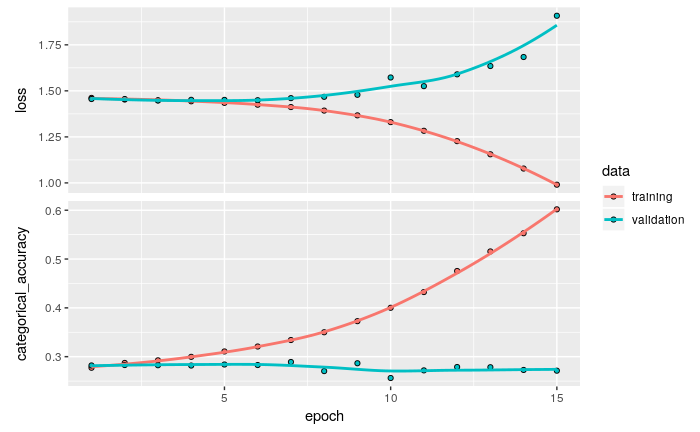
\includegraphics[width=0.8\textwidth]{./img/model1}
			\caption{Gráfica resultado del entrenamiento del primer modelo.}
			\label{first-nn}
		\end{figure}
	
		En dicha figura, para los distintos subconjuntos de datos (entrenamiento y validación), podemos apreciar varias cosas:
		
		\begin{itemize}
			\item Fase de \textbf{entrenamiento}: conforme el número de épocas aumenta, el valor de \textit{accuracy} crece y el de \textit{loss} disminuye. Esto es lo esperado, ya que manifiesta el aprendizaje de la red neuronal sobre los datos presentados en el entrenamiento, aumentando su precisión y disminuyendo el número de errores de predicción.
			\item Con respecto a la \textbf{validación}: se puede ver claramente que la \textit{precisión} se mantiene constante, mientras que el número de errores crece. Esto evidencia dos cosas: \begin{itemize}
				\item Los datos aprendidos por la red durante el entrenamiento no tienen correlación alguna con los contenidos en el subconjunto de validación, y por ello no se altera el primer valor.
				\item El algoritmo está \textit{sobreaprendiendo}; es decir, ajustándose demasiado a los datos aprendidos y no generalizando correctamente sobre aquellos nuevos que no conoce.
			\end{itemize}
		\end{itemize}
	
		A modo de última apreciación, podemos ver también en dicha figura que el valor de \textit{accuracy} en el conjunto de validación se encuentra en torno a un \textbf{26\%}, valor aproximado al que decíamos que contendría un clasificador aleatorio.
		
	\subsection{Segunda aproximación - Balanceo de clases}
	
		\begin{figure}[h]
			\centering
			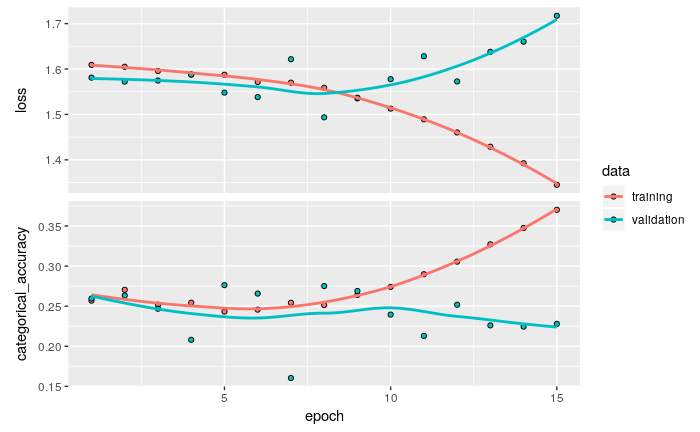
\includegraphics[width=0.8\textwidth]{./img/model2}
			\caption{}
			\label{}
		\end{figure}
	
	funciona con pesos. como tenemos los datos del histograma, podemos sacar los porcentajes (pesos) a utilizar para que estén balanceados con el resto de clases.
	
	\subsection{Tercera aproximación - \textit{Data augmentation}}
	
		\begin{figure}[h]
			\centering
			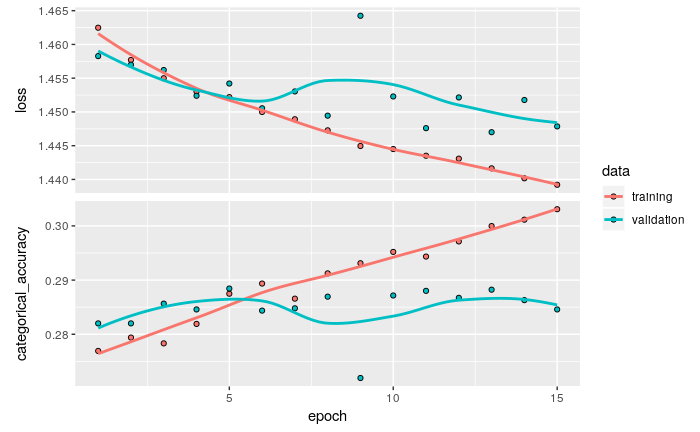
\includegraphics[width=0.8\textwidth]{./img/model3}
			\caption{}
			\label{}
		\end{figure}
	
\section{Discusión de resultados}

\section{Trabajo de investigación}

	\subsection{OVO sin balancear}
	
	\begin{table}[h]
		\begin{tabular}{lllllllllll}
			& 01 & 02 & 03 & 04 & 12 & 13 & 14 & 23 & 24 & 34 \\
			loss & 0.3481829 & 0.2762300 & 0.2932069 & 0.2874075 & 0.7930871 & 0.8128870 & 0.8359219 & 0.9399353 & 0.7924052 & 0.8011671 \\
			acc & 0.8943279 & 0.9235526 & 0.9165143 & 0.9136690 & 0.5286328 & 0.5557229 & 0.5829403 & 0.5247777 & 0.5625824 & 0.5524499
		\end{tabular}
	\end{table}
	
	\subsection{OVO balanceado}
	
	\begin{table}[h]
		\begin{tabular}{lllllllllll}
			& 01 & 02 & 03 & 04 & 12 & 13 & 14 & 23 & 24 & 34 \\
			loss & 0.5259883 & 0.5165291 & 0.5786227 & 0.5641954 & 0.8058108 & 0.7883038 & 0.7757325 & 0.8466508 & 0.7972207 & 0.7887562 \\
			acc & 0.7373737 & 0.7223159 & 0.6776356 & 0.6932636 & 0.5340014 & 0.5481928 & 0.5636792 & 0.5266836 & 0.5635705 & 0.5572809
		\end{tabular}
	\end{table}

	\subsection{OVA sin balancear}
	
	\begin{table}[h]
		\begin{tabular}{llllll}
			& 0 & 1 & 2 & 3 & 4 \\
			loss & & 0.5016596 & 0.6651614 & 0.6049633 & 0.5717794 \\
			acc & & 0.8015738 & 0.6707720 & 0.7248261 & 0.7271069
		\end{tabular}
	\end{table}
				

\section{Conclusiones}

	- el valor de accuracy hay que cogerlo con pinzas.
	- realmente el carlos está tocao de la cabeza.
	- las imágenes por sí solas no aportan información suficiente como para la resolución del problema.
	- ya estaría.

\bibliographystyle{plain}
\bibliography{sources}

\end{document}
